% !TEX spellcheck = en_US

\documentclass[conference]{IEEEtran}
\usepackage{cite}
\usepackage{amsmath,amssymb,amsfonts}
\usepackage{algorithmic}
\usepackage{graphicx}
\usepackage{textcomp}
\usepackage{xcolor}
% add hyperlinks, delete all .aux files if adding hyperref after previous build
\usepackage{hyperref}
% support for unicode charcters like "é" and "ñ"
\usepackage[T1]{fontenc}
% Provides generic commands \degree, \celsius, \perthousand, \micro and \ohm
\usepackage{gensymb}
% splits a section into multiple columns
\usepackage{multicol}
\def\BibTeX{{\rm B\kern-.05em{\sc i\kern-.025em b}\kern-.08em
    T\kern-.1667em\lower.7ex\hbox{E}\kern-.125emX}}
\begin{document}

\title{Tracker Terrain Loss Part Two}

\author{\IEEEauthorblockN{MinWah Leung, Mark A. Mikofski, Mike Hamer, Anja Neubert, Abhishek Parikh, Patrick Rainey,}
\IEEEauthorblockN{and Rounak Kharait}
	\IEEEauthorblockA{DNV, Oakland, CA, 9612, USA }}

\maketitle

\begin{abstract}
Trackers on variable terrain can incur electric mismatch losses from row-to-row shading, even with backtracking. Standard and slope-aware backtracking algorithms only eliminate row-to-row shade for trackers on flat ground. Tracker terrain loss is the difference between the theoretically best performance of trackers on flat ground and the performance of trackers using standard backtracking algorithms but on variable terrain. We used SolarFarmer to study tracker terrain loss by simulating the Hopewell Friends Solar power plant, which has an average 4\% southwest slope. We calculated a tracker terrain loss of 2.2\% when the entire site was modeled as one horizontal layout for both 5-minute and 1-hour input data. By subdividing the site into two and three layouts, the tracker terrain loss decreased to 2.0\% and 1.8\% respectively for hourly input. For this particular site, 5-minute input data did not significantly affect the tracker terrain loss, but using slope-aware backtracking completely recovered the loss. This study is a continuation of a previous study that prompted improvements in SolarFarmer's 3-dimensional tracker shading algorithm. The results of this study demonstrate that SolarFarmer can now be used to calculate tracker terrain loss. Comparison of SolarFarmer with a simpler DNV model using PVsyst produced similar results.
\end{abstract}

\begin{IEEEkeywords}
trackers, terrain, losses, backtracking
\end{IEEEkeywords}

\section{Introduction}
Trackers increase energy output of PV systems by following the sun, maximizing the area of sunlight incident on the panels. However, most silicon modules are susceptible to electrical mismatch caused by uneven shade, therefore, trackers typically "backtrack" to avoid  row-to-row shade occurring after sunrise and before sunset. The tracking and backtracking algorithms for flat horizontal and sloped ground are described by closed-form expressions \cite{Marion2013,Anderson2020}, but there is no general solution for terrain with variable slopes. If the standard backtracking algorithms for flat ground are used for trackers on variable terrain, then row-to-row shading will occur, and therefore common silicon panels will incur electrical mismatch losses. The loss has been called the "tracker terrain loss" and can be expressed as the difference between the performance of trackers on flat versus variable terrain. Evaluating the tracker terrain loss is important because it can help determine if advanced tracker algorithms are necessary to reduce the risk of plant underproduction.

To study tracker terrain loss in detail, we used SolarFarmer \cite{Mikofski_8547323} because it can perform full 3-dimensional modeling of the shade and irradiance on the trackers in any position on any terrain and calculate full sub-module electrical mismatch to determine the performance of the PV system at each time step. This study is a continuation from last year \cite{Mikofski_9300381} in which we determined that the prior methods used in SolarFarmer were too coarse to resolve row-to-row shade for trackers during backtracking. Therefore, over the past year, a new hybrid 3-dimensional geometric shade algorithm was implemented in SolarFarmer to calculate the row-to-row shade on trackers at each time step exactly without any approximations. This paper presents the results of the new SolarFarmer methods applied to the same tracker simulations from last year, and expands on them slightly by testing both standard horizontal and slope-aware backtracking algorithms and running the simulations with both 5-minute and 1-hour input data resolution to determine if the tracker terrain losses are affected by either.

\section{Methods}

\subsection{Site Characteristics}

The Hopewell Friends Solar power plant is a single-axis array funded by the Department of Energy and built by Cypress Creek Renewables \cite{CypressCreekRenewables2019} near Asheboro, NC at a latitude and longitude of 35.627994$^\circ$ and -79.872853$^\circ$ respectively. The site is asymmetric, with 25-qty variable length rows of 2-in-portrait and 18-modules wide single-axis trackers. The modules are 1.978-meters long, and the rows are spaced about 7.8-meters apart, so the GCR is about 51\%. There are 18-qty Longi LR6-72BP-360 360-watt bifacial modules per string, and three strings per each Huawei SUN2000-25KTL-US 25-kW inverter. The inverters each have three inputs, so that's one string per input.

The terrain has a generally southwestern slope as shown in the contour map in Fig.~\ref{fig:hopewell_contour_map} with slightly steeper southern slopes on the east side of the array and milder western slopes on the north side of the array. The maximum and average slopes for each aisle from west to east in the array are summarized in Table~\ref{table:ew-slope-summary} starting with aisle 1 at the top northern tip of the array. The maximum and average north-south slopes for every 5 rows are shown in Table~\ref{table:row-slope-summary} starting with the 1st row on the western side of the array.

\begin{figure}[htbp]
\centerline{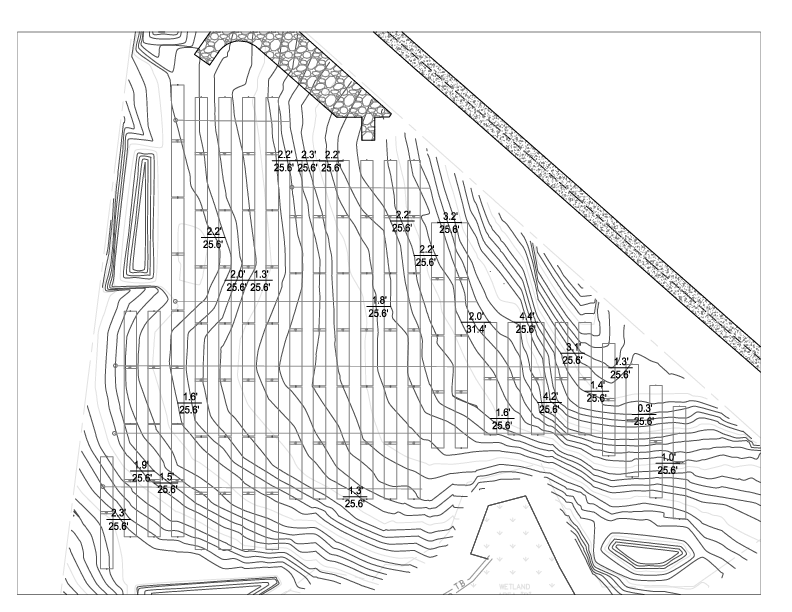
\includegraphics[width=9cm]{Hopewell_Civil_Base.png}}
\caption{Contour map of terrain at Hopewell, NC, single-axis array.}
\label{fig:hopewell_contour_map}
\end{figure}

\begin{table}[htbp]
\caption{Summary of East-West Slopes}
\begin{center}
\begin{tabular}{|c|c|c|c|}
\hline
\textbf{Aisle} & \textbf{\textit{Maximum}}& \textbf{\textit{Average}}& \textbf{\textit{Direction}} \\
\hline
1& 7.81& 6.22& west \\
\hline
2& 7.58& 6.59& west \\
\hline
3& 6.7& 5.77& west \\
\hline
4&5.99& 5.26& west \\
\hline
5& 5.08& 4.28& west \\
\hline
6& 4.69& 3.54& west \\
\hline
7& 4.42& 3.28& west \\
\hline
8& 4.06& 3.99& west \\
\hline
\end{tabular}
\label{table:ew-slope-summary}
\end{center}
\end{table}

\begin{table}[htbp]
\caption{Summary of North-South Slopes}
\begin{center}
\begin{tabular}{|c|c|c|c|}
\hline
\textbf{Row} & \textbf{\textit{Maximum}}& \textbf{\textit{Average}}& \textbf{\textit{Direction}} \\
\hline
1&  1.76&  1.11& south \\
\hline
5&  2.04&  1.77& south \\
\hline
10& 2.95&  2.54& south \\
\hline
15& 4.81&  4.35& south \\
\hline
20& 6.66&  5.84& south \\
\hline
25& 8.35&  4.96& south \\
\hline
\end{tabular}
\label{table:row-slope-summary}
\end{center}
\end{table}

\subsection{Model Simulation}

The system was modeled using SolarFarmer \cite{Mikofski_8547323} which allows parallel trackers to be oriented in any direction on any slope either in a plane or following the terrain. Trackers in SolarFarmer can backtrack on any arbitrary slope using a slope aware backtracking algorithm \cite{Anderson2020}. Normally backtracking avoids row-to-row shading while minimizing the angle of incidence to maximize output energy. However this is only true for systems constrained to a plane, and single axis trackers following the terrain may shade each other even while backtracking. As shown in Fig.~\ref{terrain-shade} row-to-row shading can occur wherever the terrain deviates significantly from the mono-plane that the trackers assume for backtracking calculations, and therefore shading can vary across the site as the terrain varies.

\begin{figure}[htbp]
\centerline{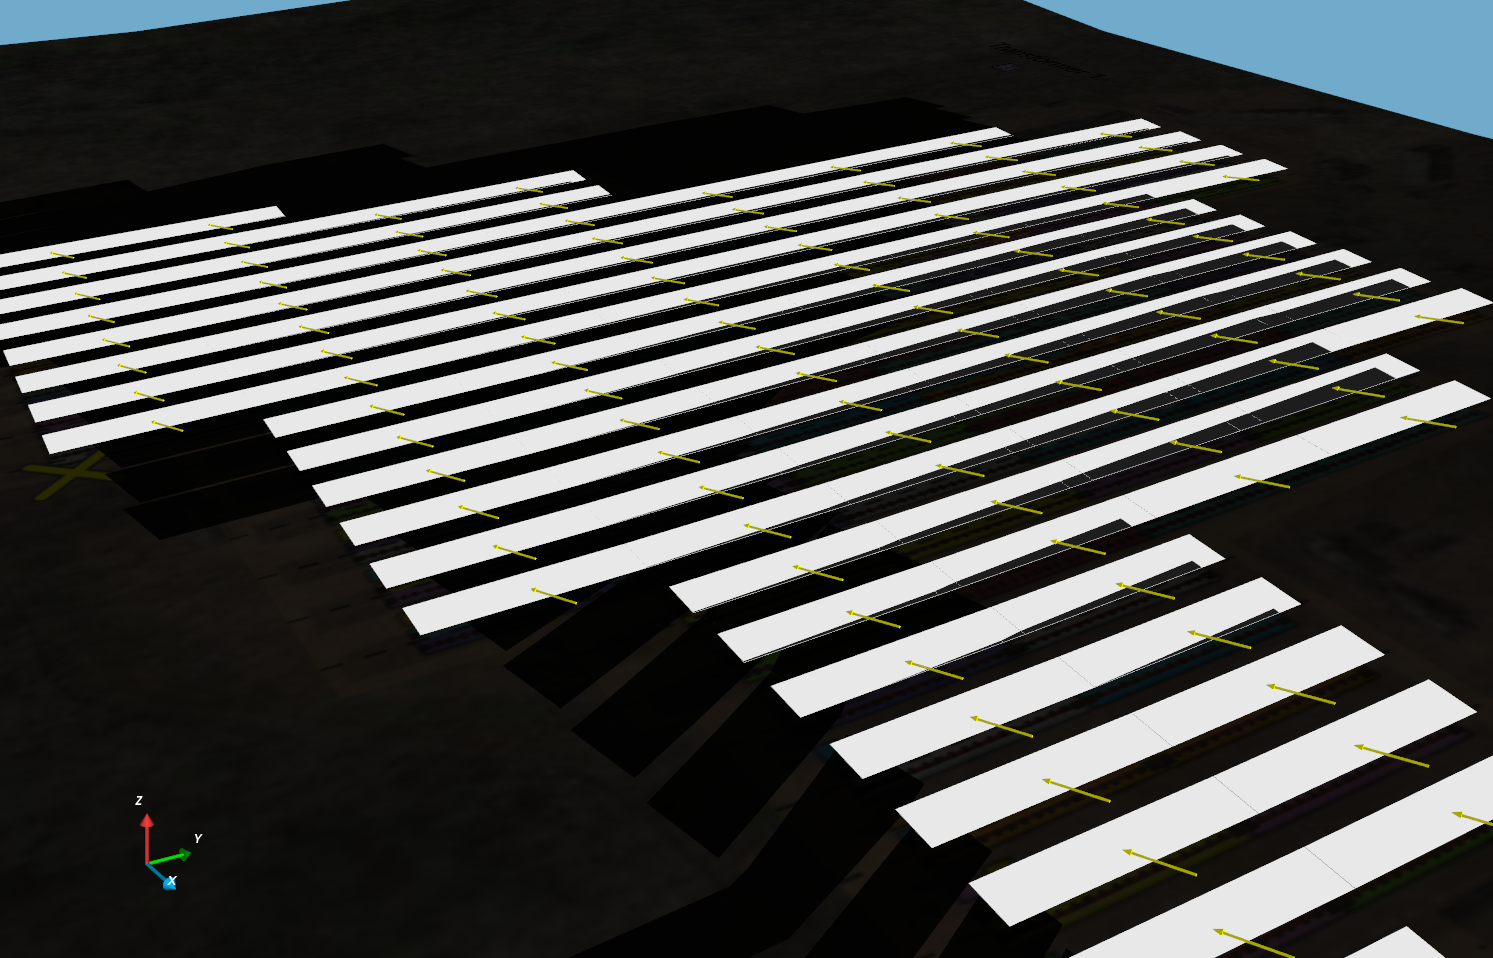
\includegraphics[width=9cm]{Hopewell-Friends-SolarFarmer-shade-follows-std.png}}
\caption{SolarFarmer simulation of row-to-row shading during backtracking for single-axis trackers following the sloping terrain at the Hopewell, NC, at 5:40 AM on June 17, 2019. Note that due to differences in north-south slopes between rows, some shadows are triangular, and therefore, shade is non-uniform accross the array.}
\label{terrain-shade}
\end{figure}

The current version of SolarFarmer offers both 2D and 3D simulations. For this study it’s necessary to use the 3D simulation to allow trackers to follow the terrain. The 3D simulation uses a combination of two techniques to calculate shading on the trackers: a geometric solution to calculate accurate row-to-row shading for the beam component, and a software rasterization approach that renders the scene on “hemicubes” located at the center of each module for the diffuse component. 

The geometric solution results in sufficient accuracy to determine shade, incident irradiance, and any electrical mismatch, and therefore the resulting energy output on trackers at any arbitrary timestep, rotation, and terrain. It does not currently consider shading from arbitrary obstacles or the terrain, but for this study there were no other shading obstacles other than the trackers themselves.

The software rasterization approach (used in the previous paper \cite{Mikofski_9300381}) is required to calculate the diffuse shading component for the trackers. Although less computationally intense than ray-tracing, the software rasterization approach is still more complex than the 2D model, so this calculation is further simplified by binning the tracker positions at all time-steps into 10° buckets, and each time-step can then be associated with a tracker position bin. The calculation then loops over the typically twelve tracker position bins and renders the full 3D scene at a representative rotation for the bin. The shading obstacles are then projected onto pixels of each hemicube, and the results are transformed into a cache of shaded or not shaded state for each 1° azimuth and zenith bin for each hemicube. These are then transformed into a diffuse component depending on how much of the sky is visible by each hemicube. A single hemicube at the center of each module was deemed sufficient to determine diffuse sky irradiance incident in the plane of array for the entire module as the view factor for diffuse sky varies very little on the front side of the module (around 8\% difference between top and bottom according to the 2D model \cite{Mikofski_8980572}). Also, when incorporating the diffuse component in the energy calculation an average of the individual module diffuse sky irradiances over the site is used per time-step, and along with approximations introduced with the tracker position binning, any finer-resolution hemicube calculations would have little effect on the result.

The combination of these two shading approaches results in a sufficiently accurate solution that runs in an acceptable computation time.

\subsection{Model Site Layouts}

The Hopewell Friends Solar array was modeled with 111-qty trackers with a total of 222 strings for a total DC size of 1.44-MW, which is slightly smaller than the specified size of 1.45-MW. Also the modeled site has 74 inverters with a DC/AC ratio less than one to remove the effects of clipping, versus the actual site which has only 45 inverters and a DC/AC ratio of 1.3. Also the simulated tracker spacing is uniform throughout the array and the tracker aisles are aligned, which also differs from the site specifications. Finally the panels were treated as monofacial, because bifacial is currently only possible for 2-dimensional simulations, and for this study we needed to take advantage of 3-dimensional modeling to capture the terrain. These changes were made for ease of modeling and to make sure that variable row spacing and other artifacts did not affect the results, since we only want to observe the effect of slope.

Fig.~\ref{fig:layouts} shows how the site was modeled three times using a single layout, 2 layouts, and 3 layouts. As shown in Table~\ref{table:system-summary}, this results in layouts with different orientations, so they will track slightly differently. Each model was then simulated in both tracker placement modes to determine the tracker terrain loss. The "in-plane" mode positions all trackers in the same plane so there is zero row-to-row shading, but may result in some trackers exceeding the maximum specified height above the ground. The "follow terrain" mode positions the trackers at the minimum specified height at which they don't intersect the ground. The "layout-plane" in Table~\ref{table:system-summary} specifies the plane of the trackers for "in-plane" mode and is the plane that determines backtracking for "follow terrain" mode. Each model was simulated with both standard \cite{Marion2013} and slope-aware \cite{Anderson2020} backtracking, and both 5-minute and hourly irradiance input, which was obtained from the NREL Physical Solar Model v3 (PSM3) \cite{Sengupta2018}. Therefore, there were a total of 24 runs, 8 for each model, with 2 placement models, 2 backtracking algorithms, and 2 input data resolutions.

\begin{figure}[htbp]
\centerline{\includegraphics[width=9cm]{layouts.png}}
\caption{Sketch of 3-layout model, layout \#2 with 30 strings is outlined in red, layout \#1 with 54 strings is to the west and layout \#3 with 27 strings is to the east. The 2-layout model combines layout \#2 and \#3 for 57 strings total, while layout \#1 remains the same.}
\label{fig:layouts}
\end{figure}

\begin{table}[htbp]
\caption{Summary Tracker Layouts}
\begin{center}
\begin{tabular}{|c|c|c|c|}
\hline
\textbf{Number of Layouts} & \textbf{\textit{1}}& \textbf{\textit{2}}& \textbf{\textit{3}} \\
\hline
number of trackers&    111& 54&  54 \\
        &     &   57&  30 \\
        &     &     &  27 \\
\hline
layout-plane azimuth (\degree)& 236.9&  247.26&  246.78 \\
       &      &  223.03&  238.47 \\
       &      &        &  207.58 \\
\hline
layout-plane tilt (\degree)&    2.83&    2.92&    2.89 \\
    &        &    2.98&    3.58 \\
    &        &        &    3.26 \\
\hline
tracker axis tilt (\degree)&   1.55&    1.13&    1.14 \\
         &       &    2.18&    1.87 \\
         &       &        &    2.89 \\
\hline
tracker side-slope (\degree)&  2.37& 2.69&    2.66 \\
          &     & 2.03&    3.05 \\
          &     &     &    1.51 \\
\hline
\end{tabular}
\label{table:system-summary}
\end{center}
\end{table}


\section{Results}

The tables in this section contain total global incident (GI) insolation in $kWh/m^2$, energy yield in $kWh/kW_p$, the percent of plane of array irradiance lost to shading, and the percent of output lost to electrical mismatch compared to the maximum power point of the array. These results are used to calculate the loss due to tracker terrain loss, which was calculated using the following formula:

\begin{equation}
\text{Tracker Terrain Loss} = 1 - \frac{Y_\text{terrain}}{Y_\text{plane}}\label{eq:tracker-terrain-loss}
\end{equation}

In (\ref{eq:tracker-terrain-loss}), $Y_\text{terrain}$ and $Y_\text{plane}$ are the energy yield in $kWh/kW_p$ of the trackers following the terrain and in a mono-plane respectively. The simulated energy yield for 5-minute input data with standard backtracking is shown in Table~\ref{table:standard-5min}. Each row refers to two simulations: in a plane and following terrain, for each of the models with either 1, 2, or 3 layouts for a total of six simulations. The calculated tracker terrain loss using (\ref{eq:tracker-terrain-loss}) is nearly zero regardless of how many layouts the site is split into because standard backtracking on sloping terrain will incur electrical mismatch as shown in Table~\ref{table:standard-5min}. Even aligning the tracker axes into mono-planes as given in Table ~\ref{table:system-summary} will still have an east-west cross-axis slope and is therefore \textit{not} horizontal. When using the standard backtracking algorithm with a westward slope, there will be shading and electrical losses in the morning because backtracking \textit{stops} too early causing row-to-row shading, and there will be irradiance losses in the afternoon because backtracking \textit{starts} too early causing cosine losses when the projected solar zenith is not normal to the plane of the array.

\begin{table}[htbp]
\caption{Energy Yield for Tracker Layouts for 5-minute Input Data with Standard Backtracking}
\begin{center}
\begin{tabular}{|c|c|c|c|c|c|}
\hline
\textbf{Lay-}& \textbf{\textit{Terrain}}& \textbf{\textit{GI}}&        \textbf{\textit{Yield}}&        \textbf{\textit{Shading}}& \textbf{\textit{Mismatch}} \\
\textbf{outs}& \textbf{\textit{Mode}}&    \textbf{\textit{$kWh/m^2$}}& \textbf{\textit{$kWh / kW_p$}}& \textbf{\textit{\%}}&      \textbf{\textit{\%}} \\
\hline
1& In Plane& 2044.0&  1628.6& 2.6& 3.4 \\
 & Follow&         &  1625.8& 2.7& 3.4 \\
\hline
2& In Plane& 2045.4&  1632.9& 2.6& 3.2 \\
 & Follow&         &  1631.8& 2.6& 3.2 \\
\hline
3& In Plane& 2046.5&  1637.1& 2.6& 3.1 \\
 & Follow&         &  1636.4& 2.6& 3.1 \\
\hline
\end{tabular}
\label{table:standard-5min}
\end{center}
\end{table}

The result that trackers following the terrain have the same loss as trackers in a plane might indicate that non-uniform shade from variable terrain has an insignificant effect on performance compared to losses from standard backtracking on sloping terrain. To study this further we compare the standard backtracking to a horizontal plane and a plane with the same axis tilt but no east-west slope. The results in Table~\ref{table:horizontal-5min} show the horizontal results, but the no east-west slopes simulations were only run for hourly results, so we'll examine those results in Table~\ref{table:no-east-west-5min}. Calculating the terrain loss using (\ref{eq:tracker-terrain-loss}) but using the horizontal plane results from Table~\ref{table:horizontal-5min} yields terrain losses of 2.2\%, 1.9\%, and 1.7\% for 1, 2, and 3 layouts respectively.

\begin{table}[htbp]
\caption{Energy Yield for Tracker Layouts for 5-minute Input Data with Standard Backtracking on Horizontal Ground or Ground with no East-West slope}
\begin{center}
\begin{tabular}{|c|c|c|c|c|c|}
\hline
\textbf{Lay-}& \textbf{\textit{Terrain}}& \textbf{\textit{GI}}&        \textbf{\textit{Yield}}&        \textbf{\textit{Shading}}& \textbf{\textit{Mismatch}} \\
\textbf{outs}& \textbf{\textit{Mode}}&    \textbf{\textit{$kWh/m^2$}}& \textbf{\textit{$kWh / kW_p$}}& \textbf{\textit{\%}}&      \textbf{\textit{\%}} \\
\hline
1& Horiz.& 2024.1&  1662.1& 3.1& 0 \\
 & No EW &       &     ---& ---& 0 \\
\hline
2& Horiz.& 2024.1&  1663.5& 3.0& 0 \\
 & No EW &       &     ---& ---& 0 \\
\hline
3& Horiz.& 2024.1&  1664.8& 2.9& 0 \\
 & No EW &       &     ---& ---& 0 \\
\hline
\end{tabular}
\label{table:horizontal-5min}
\end{center}
\end{table}

Table~\ref{table:slope-5min} repeats the simulations with slope-aware backtracking. The calculated tracker terrain losses are now significant compared to the standard backtracking case because slope-aware backtracking eliminates any row-to-row shading and electrical mismatch losses for trackers on non-horizontal planes. The tracker terrain loss using (\ref{eq:tracker-terrain-loss}) is 2.4\%, 1.9\%, and 1.6\% for 1, 2, and 3 layouts respectively. Interestingly, if the slope-aware backtracking over terrain is compared to the horizontal results in Table~\ref{table:horizontal-5min}, the tracker terrain loss is about zero. Slope-aware backtracking improves performance versus standard backtracking for the arrays over terrain by 2.0\%, 2.2\%, and 2.2\% for 1, 2, and 3 layouts respectively. So to summarize, from horizontal there is about a 2\% loss for trackers on terrain, but there's a 2\% boost from slope-aware backtracking that cancels out the tracker terrain loss.

\begin{table}[htbp]
\caption{Energy Yield for Tracker Layouts for 5-minute Input Data with Slope-Aware Backtracking}
\begin{center}
\begin{tabular}{|c|c|c|c|c|c|}
\hline
\textbf{Lay-}& \textbf{\textit{Terrain}}& \textbf{\textit{GI}}&        \textbf{\textit{Yield}}&        \textbf{\textit{Shading}}& \textbf{\textit{Mismatch}} \\
\textbf{outs}& \textbf{\textit{Mode}}&    \textbf{\textit{$kWh/m^2$}}& \textbf{\textit{$kWh / kW_p$}}& \textbf{\textit{\%}}&      \textbf{\textit{\%}} \\
\hline
1& In Plane& 2044.9&  1700.0& 1.9& 0 \\
 & Follow&         &  1658.9& 2.1& 2.1 \\
\hline
2& In Plane& 2046.3&  1700.3& 1.9& 0 \\
 & Follow&         &  1668.3& 2.0& 1.7 \\
\hline
3& In Plane& 2047.3&  1701.8& 1.9& 0 \\
 & Follow&         &  1673.9& 2.0& 1.5 \\
\hline
\end{tabular}
\label{table:slope-5min}
\end{center}
\end{table}

Table~\ref{table:standard-1hr}, Table~\ref{table:no-east-west-5min}, and Table~\ref{table:slope-1hr} show results for both backtracking algorithms with hourly input data. There are very small increases in output and global incident irradiance compared to the 5-minute input that we believe are because 5-minute input more accurately captures backtracking which often occurs over only part of an hour. We will present a separate study to examine this issue more closely later this year.

\begin{table}[htbp]
\caption{Energy Yield for Tracker Layouts for 1-hour Input Data with Standard Backtracking}
\begin{center}
\begin{tabular}{|c|c|c|c|c|c|}
\hline
\textbf{Lay-}& \textbf{\textit{Terrain}}& \textbf{\textit{GI}}&        \textbf{\textit{Yield}}&        \textbf{\textit{Shading}}& \textbf{\textit{Mismatch}} \\
\textbf{outs}& \textbf{\textit{Mode}}&    \textbf{\textit{$kWh/m^2$}}& \textbf{\textit{$kWh / kW_p$}}& \textbf{\textit{\%}}&      \textbf{\textit{\%}} \\
\hline
1& In Plane& 2049.9&  1628.9& 2.8& 3.6 \\
 & Follow&         &  1631.1& 2.6& 3.6 \\
\hline
2& In Plane& 2051.5&  1635.0& 2.7& 3.4 \\
 & Follow&         &  1635.9& 2.6& 3.4 \\
\hline
3& In Plane& 2052.7&  1639.8& 2.6& 3.2 \\
 & Follow&         &  1640.3& 2.6& 3.2 \\
\hline
\end{tabular}
\label{table:standard-1hr}
\end{center}
\end{table}

The tracker terrain losses calculated with (\ref{eq:tracker-terrain-loss}) for the standard-backtracking cases in Table~\ref{table:standard-1hr} are close to zero as they were for the 5-minute input. Therefore, as with the 5-minute input, we compare the arrays over terrain to arrays constrained to a horizontal plane and to a plane with an axis tilt but no east-west slope in Table~\ref{table:no-east-west-5min}. Compared to horizontal, arrays over terrain using standard backtracking had tracker terrain losses of 2.2\%, 2.0\%, and 1.8\% with 1, 2, and 3 layouts respectively. However, this site has a south-facing slope that adds a tilt-gain, because the site is in the northern hemisphere, so the sun is to the south. If we compare the array over terrain to an array constrained to a plane with a southern axis tilt but no east-west slope, we get a tracker terrain loss of 4.5\%, 4.0\%, and 3.9\%. Therefore for this particular site with southwest sloping terrain, comparing the performance of the array on terrain versus horizontal underestimates the tracker terrain loss, because it disregards the tilt-gain from the the southern axis tilt.

\begin{table}[htbp]
\caption{Energy Yield for Tracker Layouts for 1-hour Input Data with Standard Backtracking on Horizontal Ground or Ground with no East-West slope}
\begin{center}
\begin{tabular}{|c|c|c|c|c|c|}
\hline
\textbf{Lay-}& \textbf{\textit{Terrain}}& \textbf{\textit{GI}}&        \textbf{\textit{Yield}}&        \textbf{\textit{Shading}}& \textbf{\textit{Mismatch}} \\
\textbf{outs}& \textbf{\textit{Mode}}&    \textbf{\textit{$kWh/m^2$}}& \textbf{\textit{$kWh / kW_p$}}& \textbf{\textit{\%}}&      \textbf{\textit{\%}} \\
\hline
1& Horiz.& 2029.6&  1668.7& 3.1& 0 \\
 & No EW & 2049.9&  1707.2& 1.8& 0 \\
\hline
2& Horiz.& 2029.6&  1670.0& 3.0& 0 \\
 & No EW & 2051.5&  1703.9& 2.1& 0 \\
\hline
3& Horiz.& 2029.6&  1671.4& 2.9& 0 \\
 & No EW & 2052.7&  1706.3& 2.0& 0 \\
\hline
\end{tabular}
\label{table:no-east-west-5min}
\end{center}
\end{table}

When slope-aware backtracking is used, the tracker terrain losses using (\ref{eq:tracker-terrain-loss}) for the results in Table~\ref{table:slope-1hr} are 2.5\%, 1.9\%, and 1.7\% for 1, 2, anr 3 layouts respectively. Even more interestingly, we see by comparing Table~\ref{table:slope-1hr} and Table~\ref{table:no-east-west-5min} that slope-aware backtracking for the in-plane array was about the same as standard backtracking on the no east-west plane, and also as with the 5-minute input, we see that trackers over terrain with slope-aware backtracking perform about as well as trackers in a horizontal plane with standard backtracking. So this even further confirms that slope-aware backtracking eliminates the losses from east-west slopes. Compared to standard backtracking, slope-aware backtracking for trackers over terrain improves performance by 1.9\%, 2.2\%, and 2.3\% for 1, 2, and 3 layouts respectively. This is consistently about the same as the tracker terrain loss for this particular site with a southwest slope. Therefore, it seems that the east-west slope is the main cause of tracker terrain losses at this particular site, and that slope-aware backtracking seems to recover those losses. Furthermore, when comparing the best output from an in-plane array with slope-aware backtracking to the worst output from standard backtracking over terrain, the loss is 4.3\%, 4.1\%, and 3.9\%. Again, we see that comparing the performance of the array over terrain to the horizontal case underestimates the tracker terrain loss because it fails to account for the terrain in both directions, it fails to capture tilt-gain from the southern axis tilt, and it only accounts for the loss from the east-west slope. Basically it only accounts for the inability of standard backtracking to account for cross-axis slope.

\begin{table}[htbp]
\caption{Energy Yield for Tracker Layouts for 1-hour Input Data with Slope-Aware Backtracking}
\begin{center}
\begin{tabular}{|c|c|c|c|c|c|}
\hline
\textbf{Lay-}& \textbf{\textit{Terrain}}& \textbf{\textit{GI}}&        \textbf{\textit{Yield}}&        \textbf{\textit{Shading}}& \textbf{\textit{Mismatch}} \\
\textbf{outs}& \textbf{\textit{Mode}}&    \textbf{\textit{$kWh/m^2$}}& \textbf{\textit{$kWh / kW_p$}}& \textbf{\textit{\%}}&      \textbf{\textit{\%}} \\
\hline
1& In Plane& 2048.7&  1704.7& 1.9& 0 \\
 & Follow&         &  1662.1& 2.1& 2.2 \\
\hline
2& In Plane& 2050.2&  1705.0& 2.0& 0 \\
 & Follow&         &  1672.3& 2.1& 1.8 \\
\hline
3& In Plane& 2051.1&  1706.4& 1.9& 0 \\
 & Follow&         &  1678.1& 2.0& 1.5 \\
\hline
\end{tabular}
\label{table:slope-1hr}
\end{center}
\end{table}

The last component of this study was to examine the hypothesis that splitting the array into multiple layouts each with their own axis tilt and cross-axis slope would decrease tracker terrain loss. We see that in general, for this particular site, splitting the site into 3 layouts increased performance and decreased the tracker terrain loss by about half a percent of the output. More importantly, if maximum performance is desired, then in-plane trackers are required, and splitting the array into layouts each with their own axis tilt and cross-axis slope can minimize the amount of cut and fill required to build the site by decreasing the range of pile heights to constrain the tracker axes all to the same plane.

\section{Conclusions}
The Hopewell Friends Solar power plant was simulated with SolarFarmer to calculate tracker terrain loss. This site has variable terrain and an average 4\% southwest slope. When using standard backtracking the tracker terrain loss for the entire site was 2.2\% when compared to horizontal and using hourly input. When dividing the site into two and three layouts, the tracker terrain loss decreased to 2.0\% and 1.8\% respectively. The simulations were repeated with 5-minute and 1-hour input data, but the tracker terrain loss change was marginal. A future study will examine the effects of input data resolution and backtracking algorithms. The simulations were also repeated with slope-aware backtracking algorithm, which indicated that for this particular site, the tracker terrain loss was caused by the east-west slope and was completely recovered by using slope-aware backtracking. Furthermore, the maximum gain was around 4\% when comparing trackers on terrain to an in-plane array using slope-aware backtracking, indicating that calculating tracker terrain loss against the horizontal for this particular site neglected the tilt-gain from south-facing slope.  Since this site had a mostly southwest slope, further work is needed to study many more sites, especially those with more complex or rolling terrain.

\section*{Acknowledgment}

Data and layout specifications for the Hopewell Friends Solar array were provided by PV Evolution Labs and Cypress Creek Renewables based on funding by the U.S. Department of Energy office of Energy Efficiency and Renewable Energy as detailed in the funding opportunity announcement, DE-FOA-0001840 \cite{CypressCreekRenewables2019}.

\bibliographystyle{IEEEtran}
% argument is your BibTeX string definitions and bibliography database(s)
\bibliography{IEEEabrv,bibliography}

\end{document}
